\chapter{Background}
Creating a cyborg is a massive cross disciplinary effort, and if a scope is not
clearly defined the background runs the risk of becoming equally massive.
The goal of the thesis is to create a hybrid neuro-digital system capable of
controlling a simple robot, and by extension to create a ``bridge'' between
neural and digital.
Each section in the background shares this bridge as a red thread, and
consequently topics that are not directly related to the thesis' goal are discarded.
The background is laid out as follows:
First \emph{Complex Systems} are introduced as a framework to discuss the computational
capabilities in a wide range of systems that exhibit system dynamics similar to
that of neurons.
Modeling neurons as a complex systems is a first step towards establishing a
common ``language'' between neural activity and digital logic.
%
Next, \emph{Evolution in Materio}, EiM for short, introduces computation done in
unstructured matter through the process of evolution.
The goals of EiM are closely aligned to the goal of this thesis, as both study
massively parallel computation happening in physical matter shaped by the
process of evolution.
%
Next section, \emph{Neurons As Computers} introduces neurons with a strong focus
on their computational capabilities.
Building on the EiM section, this section motivates a necessary reduction of
scope, proposing a simplified model of the computing neuron and a medium of
communication between neuron and digital.
%
Finally, \emph{Reservoir Computing} is introduced, tying together the previous
sections by introducing the framework of reservoir computing in order to
establish a common ``language'' between neural cultures and digital.
\section{Complex Systems}
% TODO: Introduser Adaptive networks, siter Sayama: "Modeling complex systems with
% adaptive networks"
%
% How nature deals with CX:
When designing systems in a top down manner it is imperative to control the
complexity of the system, or we are unable to reason about what it does and how
it does so.
By carefully managing complexity it is possible to make systems that are
\emph{complicated} in their makeup, yet with a simple, understandable behavior.
Larger systems can be assembled by combining smaller systems, and since each
subcomponent acts in a simple, predictable way, then so does the system as a
whole.
The effort necessary to understand the behavior of system as a whole is the same
as the sum of the effort required to understand each of its subsystems, and so
forth.
%
When studying most systems that occur naturally however, such as economical
systems, ecosystems, materials and how neurons together make up the mind, this
does not hold.
%
This is because the behavior we would like to model and predict cannot be traced
back to the individual agents of the system.
%
Although the individual parts of these \emph{Complex Systems} can be just as
complicated as in human engineered ones, it is the \emph{Non-linear} dependence
between these parts that decides the behavior of the system as a whole.
%
It is these complex interactions that allows systems to spontaneously \emph{Self
  Organization} and adapt to change.
%
The ``force'' that drives the self organization of complex systems is feedback.
Positive feedback loops can cause a chain reaction that completely alter the
dynamics of a system, while negative feedback acts as a dampener, allowing the
system to have some measure of stability.
Systems with mostly negative feedback are ordered and predictable, while systems
with mostly positive feedback are chaotic and unpredictable, seemingly random.
It is at \emph{The edge of chaos} where positive and negative feedback are
evenly matched that systems can spontaneously self organize without being chaotic.
%
In the context of evolution seems necessary for systems to exist at this edge of
chaos.
For a plant it is essential to be able to respond to changes in light
conditions, but it is equally important to maintain integrity.
No two pines are alike, but they all have bark on the outside and they all grow
upwards.
In a swiss watch everything stops working if a single spring or cog is replaced
with a slightly different one, yet in nature no two animals or plants are alike.
The \emph{robustness} of complex systems goes beyond mere survival, it's what
makes the incremental changes of evolution possible in the first place!
%
While the neurons that make up neural networks are both complex and complicated,
it is in the interactions between them that computation happens, and this
complex interaction can be modeled in a much simpler system.
\par
\begin{figure}[h!]
  \centering
  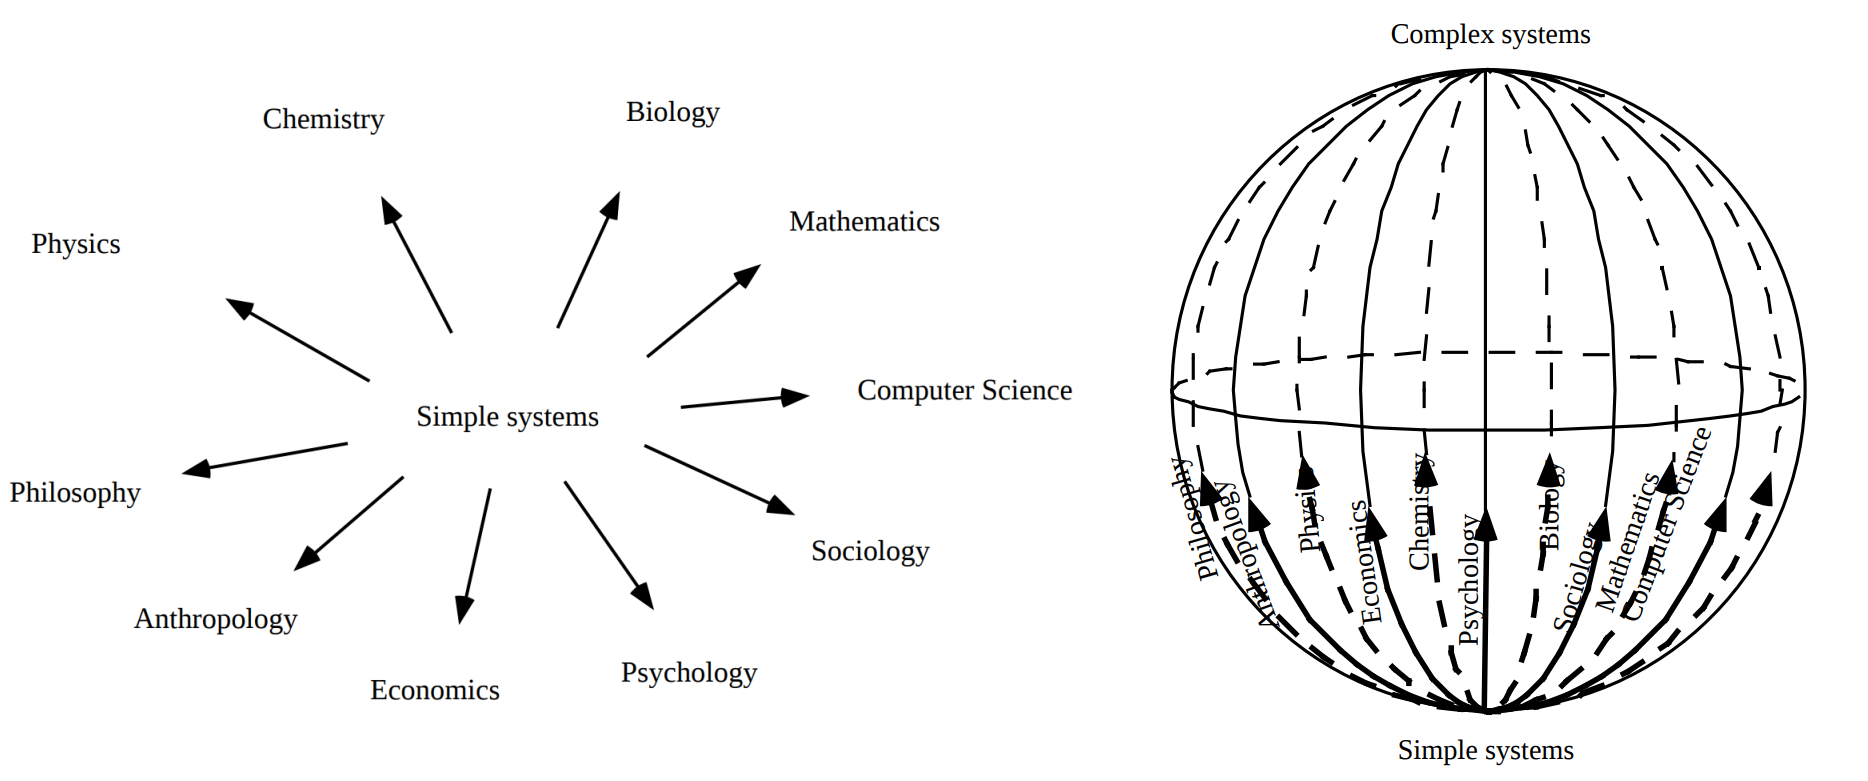
\includegraphics[width=0.6\textwidth]{fig/BarYamCX.png}
  \caption{From Bar Yam book.}
  \label{figCX}
\end{figure}
% CA: Intro
% Wolfram: claims of computational powers
% Langton: phase transitions
% Sipper: not really necessary?
\subsubsection{Cellular Automata}
A \emph{Cellular Automaton}\footnote{Singular: Automaton, Plural: Automata}, CA
in short, is a simple discrete model of a single cell which changes between a
discrete set of states based only on its immediate neighbors.
Figure \ref{figCA22} shows an example of a \emph{rule set}, or \emph{transition
  table} for a cellular automaton with only two states, and an initial
configuration, or ``seed'', which over several steps forms a pattern.
%
One of the pioneers in the field of CAs, Stephen Wolfram suggested that under
certain conditions CAs were capable of computation [cite Wolfram: Universality
and complexity in cellular automata].
%
Cellular automatas have been shown capable of solving global problems such as
contour-extraction \cite{sipper_emergence_1999} where the problem is expressed
as the seed and a global solution emerges from the local interaction of cells.
Wolframs hypothesis of universal computation has also been proven correct, in
fact even a simple 1D cellular automata such as in \ref{figCA22} has been proven
sufficient to simulate a turing machine [Cite Matthew Cook],
but as Sipper puts it: ``This is perhaps the quintessential example of a slow
bullet train: embedding a sequential universal Turing machine within the
highly parallel cellular-automaton model.''\par
% 
% Her var jeg. Skriv noe om at vi tar det for gitt at utregning kan skje, vi
% bryr oss ikke om hvordan, men hva slags conditions kreves per Langton.
%
In figure [figur av class 1 - IV CA] four cellular automatas are shown,
each classified per Wolframs CA classification.
The fourth class which ``yields complex patterns of localized
structures'' shows complex behavior which Wolfram suggested was the sort of
behavior necessary for computation to occur spontaneously.
%
As a model for neurons it is sufficient to know that they are capable of
computation and under which circumstances rather than knowing exactly what they
are computing.
%
In Langton's pioneering paper \emph{Computation on the Edge of Chaos}
\cite{langton_computation_1990} the space of possible transition tables for one
dimensional cellular automata with two states, such as \ref{figCA22} is explored.
What Langton discovered was that the ratio between states leading to life and
death (black and white cells respectively) was analogous to how temperature
causes phase changes in materials.
This is not suprising, as one would expect rulesets where most transitions lead
to death will lead to a stationary system analogous to ice, while a transition
table favoring life and death equally leads to a chaotic system analogous to a
gas.
What was suprising however, was that at the edge between periodic and chaotic
there existed a \emph{Critical Phase}, shown in \ref{figCAegg}.
This effect also happens in materials in what is called a 2nd order phase
change, in which the material is neither gas, liquid or solid, but exhibits all
three in local substructures that can be found on all scales, from macroscopic
to microscopic.
The takeaway from the model of cellular computation is the idea that there are
certain criterias that enable computation to occur spontaneously, and that
neurons actively attempt to reach this critical phase.
\begin{figure}[h!]
  \centering
  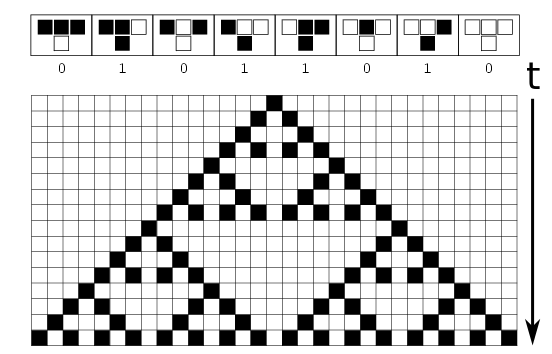
\includegraphics[width=1\textwidth]{fig/ca22.png}
  \caption{Should add a time axis to drive the point home that these are 1D}
  \label{figCA22}
\end{figure}
\begin{figure}[h!]
  \centering
  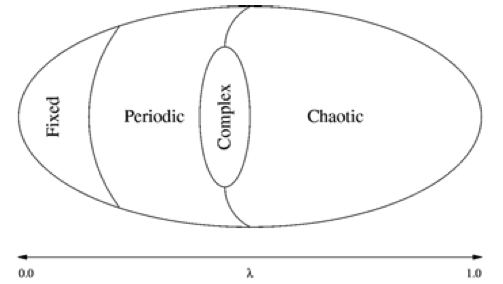
\includegraphics[width=1\textwidth]{fig/Langtons_egg2.png}
  \caption{Langtons egg}
  \label{figCAegg}
\end{figure}

% but where is the evolution?
\section{Evolution In Materio}
Modeling neurons as cellular automata gives an idea of how neurons organize
themselves into computationally capable networks and how this computation may
look like, but the question of how to make sense of these dynamics and utilize
them.
Before tackling neurons it is necessary to extend our model to the physical
realm and develop a model that can be extended to perform computation.
A very natural extension of the CA model is \emph{material computing} in which
the atoms that make up matter locally interact in similar ways to CAs.
%
Two pioneers in this field were the british duo Pask and Beer which studied how
unstructured matter could be used to perform computational tasks.
%
In one experiment [cite ???] the duo used silver in an acidic solution which
would form short-lived silver filaments when subjected to electric currents.
%
By tuning the various knobs controlling parameters such as voltage this solution
could be made to perform the task of tone discrimination, proving that
unstructured matter could in fact perform computation.
%
In Langtons CAs the goal was not to compute, but to explore what conditions were
necessary for computation to occur, while Gordon and Pask sought to actually
compute by observing how the matter reacted to sound and tuning the parameters
in response.
%
Tommaso Toffoli argues that ``Nothing makes sense in computing except in the
light of evolution'' in his eponymous paper [cite TT], which separates Langtons
compute capable CAs and the tone discrimination which had been evolved by
repeatedly observing its performance and altering the parameters accordingly.
%
% Hmm hmm hmm
A corollary of the turing completeness of cellular automatas is that CAs can be
``tuned'' in a rather heavy handed way to compute, but a more interesting
conjecture is that a CA with a random seed will eventually exhibit local
self-replicating behavior, spontaneously giving rise to what Toffoli would
regard as computation, or possibly even as life.\par
%
Whereas the pioneers in material computing sought to perform specific tasks with
their experiments more recent work has been made for general computation.
One approach is \emph{Evolution In Materio} where various materials have their
parameters tuned algorithmically to perform a transformation between input and
output.
A recent effort is the NASCENCE project which has developed a physical device,
``mecobo'' that can host a variety of materials which can then be interacted
with using an array of electrodes.
By using the same basic loop as the early material computing reasearchers the
Mecobo board has been used to create XOR logic gates using unstructured carbon
nano-tubes [Cite Odd paper 1].

TODO: mer her? fikse citations.
\section{Neurons As Computers}
It is tempting to reuse the same methodology employed in EiM for neurons but
this line of thinking neglects the fact that neurons have already been shaped by
the process of evolution over billions of years.
Neurons are not unstructured matter, that can be coaxed into computing by
tweaking parameters, rather they are the result of an EiM billion years in the
making.
While directly modifying the property of matter a la EiM is not a good fit for
neural cultures there is still many clues on how to approach neurons:
When Pask and Beer tweaked their silver solution to discriminate tones, they did
viewed the solution as a black box, and only its performance on the task at hand
was evaluated.
Just like Pask and Beer did not consider the exact inner workings of silver
filaments, the monumentally complex chemical pathways and genetic regulation
that govern the growth and functionality of neural networks can be abstracted
away.
On a more theoretical level, if we imagine that the neuron were the result of an
EiM experiment, what sort of behavior did the experimenters target when varying
the parameters?
While this is not the case it does...
% TODO finish

% TODO shift focus towards the why's given previous changes.
\subsubsection{Neurons}
The neuron, or nerve cell, is the basic building block of both the human brain
and the nerve system.
There are many types of neurons in the human body, but to reduce the scope the
focus of this thesis is a simplified model of the neurons that make up the
brain.
The model neuron, shown in fig [a figure of a neuron] consists of three parts:
The body, \emph{Soma}, the \emph{Dendritic network} and an \emph{Axon}.
The dendritic network acts as a receptor sensing electrical activity around the
neuron, while the axon transmits electric pulses to neighboring cells.
The connection between two neurons is called a \emph{Synapse}.
Axons and dendritic networks are themselves vastly complex, and viewing them as
simple electrical transmitters neglects the importance of neurotransmitters.
However, given the strong correlation between neurotransmitter concentrations and
electrical activity is considered part of the black box.
When the neuron is sufficiently excited by electrical activity it will fire an
electrical pulse that travels along the axon, which in turn stimulate other
neurons.
Together neurons form networks in a complex interplay between topology and behavior:
The behavior of the network decides its behavior, and the behavior in turn
causes some synapses to wither, and others to form in a process that is not well
understood.
The model used for the neuron for the rest of this paper is a node in an
\emph{Adaptive Network} which communicates through electrical pulses.
The missing part in our model is the underlying rules that dictates the growth
of the network.
% What about spike trains?

% TODO: redo
\section{Reservoir Computing}
So far we have arrived at a model of the neuron as a complex adaptive network
which can be interfaced with using electrical signals, but the fundamental issue
of actually utilizing neurons for computing remains.
%
The final piece of the puzzle comes in the form of \emph{Reservoir Computing}, a
technique developed to exploit the dynamics of complex systems.
If the fundamental rule governing the neuron is to create networks exhibiting
the same complexity behavior as Langton's automatas then harnessing the
computational capabilities of these simple models is a first step towards
interfacing and understanding neurons.
%
% Clearly designing a cellular computer in a top down manner is intractable due to
% the intricate and unpredictable relation between cause and effect.
% The best we could realistically achieve with the typical top down approach is
% implementing a turing machine which would be both slow and incredibly brittle.
% Seemingly, classifying the neural culture as a complex system has not provided
% any useful tools for understanding how to interact with it, on the other hand it
% makes this task seem futile.
% However, in computer science the recent field of
% \emph{reservoir computing} has emerged, embracing the complexity and unpredictability
% of certain complex systems.
In reservoir computing, a complex systems is used as a \textit{reservoir}
\cite{schrauwen_overview_2007} which
``acts as a complex nonlinear dynamic filter that transforms the
input signals using a high-dimensional temporal map, not unlike the operation
of an explicit, temporal kernel function.''\\
% cite on SVMs?
In order to explain, schrauwen makes a comparison to the the machine learning
technique of source vector machines work, as shown in fig [rm 1]:
The reservoir acts as a kernel, projecting input into a high-dimensional feature space.
Figure [rm 1] shows this technique, note that the regression performed upon the
feauture space is a simple linear regression, an important point both in SVMs
and reservoir computing.
%
Figure [rm 2] shows a typical reservoir computing setup which follows a similar
method of operation as the SVM in figure [rm 1]
The reservoir serves as the high dimensional feature space, while the output
layer is only capable of linearly separating the resulting dynamics.
%
Schrauwen points out two major differences between SVMs and RCs.
First, SVMs only implicitly expands the input to high dimensional space in order
to make the problem tractable, while reservoirs do not.
Secondly, kernels are not capable of handling temporal signals.
%
The second difference is very important, it is what allows reservoirs to
implicitly encode temporal signals in their dynamics, making reservoirs a
natural fit for tasks such as speech recognition.
% cite Biologically Plausible Speech Recognition with LSTM Neural Nets Alex
% Graves, Douglas Eck, Nicole Beringer, Juergen Schmidhuber
% 
In other terms, the properties that make complex systems so hard to work with
such as sensitivity to initial conditions also allow them to discern very subtle
nuances in input, and their complex behavioral patterns causes the systems to
change their behavior to new input based on previous input.
%
In light of this, asking how to build a computer using Langton's automatons is
the wrong question, instead the focus should be on how exploit the computation
that is already occuring.\\
There are many examples of reservoirs which have been successfully exploited:
In \cite{jaeger_adaptive_2003} an \textit{echo state network} 
is utilized to solve classification problems.
More esoteric reservoirs have been used, for instance in
\cite{natschlager_liquid_2002} the idea of reservoir computing is taken quite
literally using a bucket of water as a reservoir.\\

\subsection{Linear and nonlinear output layers}
TODO: Elaborate on the use of linear vs nonlin classifiers.

\cleardoublepage

%%% Local Variables:
%%% mode: latex
%%% TeX-master: "../main"
%%% End: